\documentclass[11pt,a4paper]{article}
\usepackage[margin=2.1cm]{geometry}
\usepackage[T1]{fontenc}
\usepackage[utf8]{inputenc}
\usepackage{lmodern}
\usepackage{graphicx}
\usepackage{booktabs}
\usepackage{array}
\newcolumntype{L}[1]{>{\raggedright\arraybackslash}p{#1}}
\usepackage{longtable}
\usepackage{xcolor}
\usepackage{enumitem}
\usepackage{microtype}
\usepackage[hyphens]{url}
\usepackage[hidelinks]{hyperref}
\setlength{\parskip}{4pt}
\setlength{\parindent}{0pt}
\newcommand{\fp}[1]{{\small\path{#1}}}
\graphicspath{{figs/2026-08-30-nn-progress/}}

\title{The neural-network bot for Troll Farm\\[2pt]\large Where the project stands on 2026-08-30}
\author{Prepared for the owner by the coordinator (\texttt{local\_claude\_1})}
\date{2026-08-30, 06:1xZ --- everything below is on \texttt{main} unless a path says otherwise}

\begin{document}
\maketitle

\section*{In one page}

\textbf{The goal.} A bot for the CodinGame game \emph{Troll Farm} whose every command comes from a small neural network --- the way the \#1 player on the ladder (\emph{delineate}, rating 30.9) plays. Our best hand-written bot (``the champion of record'') reads about 18--21 on the same ladder.

\textbf{The target you set (2026-08-29).} A network candidate that beats the champion of record \emph{and} the ``orchard~6'' bot on our own bench --- at least 60\,\% wins over 400 games against each, three checks in a row --- exported as one Rust file under 100,000 characters at $\le 15$\,ms a turn, verified, ready for the ladder, \textbf{by 2026-10-17}. Milestone for your read: the clone playing whole games against the champion's file, aimed at 2026-09-14.

\textbf{Where we are, 36 hours later.}
\begin{itemize}[nosep,leftmargin=1.4em]
  \item The training environment (a full copy of the game that plays 128 games at once) is built, tested and reproduced by a second agent.
  \item Every recorded game of the top four players has been turned into a training set: \textbf{817,811 decisions from 748 games}, 14\,MB.
  \item A first network, \textbf{the clone}, learned by copying those decisions. It plays complete, legal games and \textbf{beat the champion's own file in 9 of 48 games} (134 points to 186 on average) --- \emph{the milestone, reached two weeks early.} Its games are on file for you (Section~\ref{sec:read}).
  \item \textbf{Self-play training started at 04:45Z today} from the clone. After the first hour its win rate against its practice opponents rose from 0\,\% to 39\,\%.
\end{itemize}

\textbf{What is next.} The self-play run takes about 3.5 days. Every few hours I test its latest snapshot against the champion's file; when a snapshot wins more than 55\,\% of 48 games, the card's full 400-game checks begin. Then: the export to a single Rust file, the timing and size checks, and --- on your word, when the platform is free --- one hour on the ladder.

\section{The plan and its status}

The work is one card, \fp{coordination/tasks/20260829-nn-bot-way-b.md}, in five phases. Each phase has a ``done'' condition, a ``dead'' condition and a budget, like every card on the board.

\begin{center}\small
\begin{tabular}{@{}L{0.5cm}L{6.0cm}L{2.4cm}L{6.3cm}@{}}
\toprule
 & what & budget & status \\
\midrule
0 & the software runtime on this computer; the old (July) pipeline re-run end to end & 1--2 days & \textbf{done} 08-29 14:2xZ \\
1 & the full-game training environment (Rust), with a Python wrapper & 6 days & \textbf{done} 08-29 21:1xZ, in one day; reproduced \\
2 & the training set, the bench (our judge), the clone & 7 days & \textbf{tools done and reproduced} 08-30 03:2xZ; \textbf{the clone's games on file} 04:5xZ --- the milestone \\
3 & self-play training from the clone, with checks every few days & 2--4 weeks & \textbf{running} since 08-30 04:45Z \\
4 & export to one Rust file, the timing and size checks, one ladder hour & 3 days + 1 hour & not started; waits for a candidate and for the platform \\
\bottomrule
\end{tabular}
\end{center}

\section{What was done, step by step}

\subsection*{2026-08-29 --- the analysis and your decisions}
I read what the repository already knew: the \#1 player's own description of his network (we hold his text), our July attempts at learning (they stopped for reasons that are now avoided), the game engine's speed and accuracy, the recorded games. Conclusion: every piece existed except the assembly. You decided: open the line; way B --- \emph{copy the top players first, then improve by self-play}; you judge the clone's games yourself.

\subsection*{2026-08-29 --- the environment (Phase 1)}
\emph{codex\_1} built the environment on the VM in a day. Its written interface (what the network sees, how commands are encoded, how a turn is split into decisions) was audited the same day by \emph{chatgpt\_1}, on your instruction, and \textbf{ten real defects} were found and fixed before any number was accepted --- among them: the starting troll was created with the wrong strength on both sides of the test, so the test could not have caught it; a counter of illegal commands that could never be non-zero; a check of \emph{whether} a game was replayed right but not \emph{when} it ended; and a vocabulary of buyable trolls copied from delineate that the other top players do not respect (see Section~\ref{sec:data}). The final version passed its check --- 1,000 self-play games replayed through an independent copy of the rules with no disagreement --- and \emph{claude\_1} reproduced it byte for byte.

\subsection*{2026-08-29/30 --- the training set, the bench, the clone (Phase 2)}
\emph{claude\_1} built the three tools; \emph{codex\_1} reproduced them; I ran the training set on this computer (1 minute 42 seconds) and trained the clone (4 passes over the data, 2 hours). The bench --- the clone against the champion's actual submitted file, on 24 real ladder maps, once on each side --- gave the milestone numbers. Figures~\ref{fig:clone}--\ref{fig:bench}.

\subsection*{2026-08-30 --- self-play (Phase 3)}
Started at 04:45Z on this computer from the clone: the network plays 128 games at once against six of our hand-written bots and against frozen copies of itself, on all 24,973 real ladder maps, and is nudged toward what wins, while a leash (``the anchor'') keeps it close to the clone at first. Figure~\ref{fig:ppo} is the run as of this report.

\begin{figure}[h]\centering
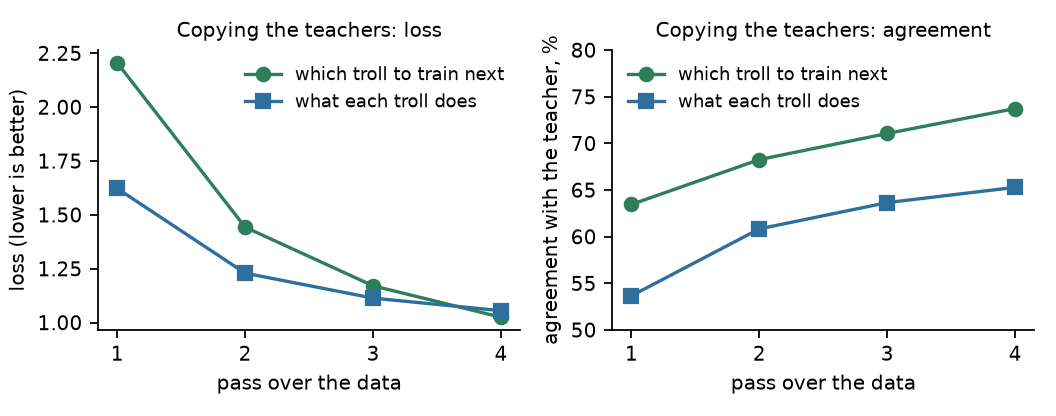
\includegraphics[width=\textwidth]{clone-epochs.png}
\caption{The clone learning to copy the teachers. Left: the loss (an error measure) of its two decisions --- which troll to save for, and what each troll does --- over the four passes. Right: how often it agrees with the teacher on the training moves.}
\label{fig:clone}
\end{figure}

\begin{figure}[h]\centering
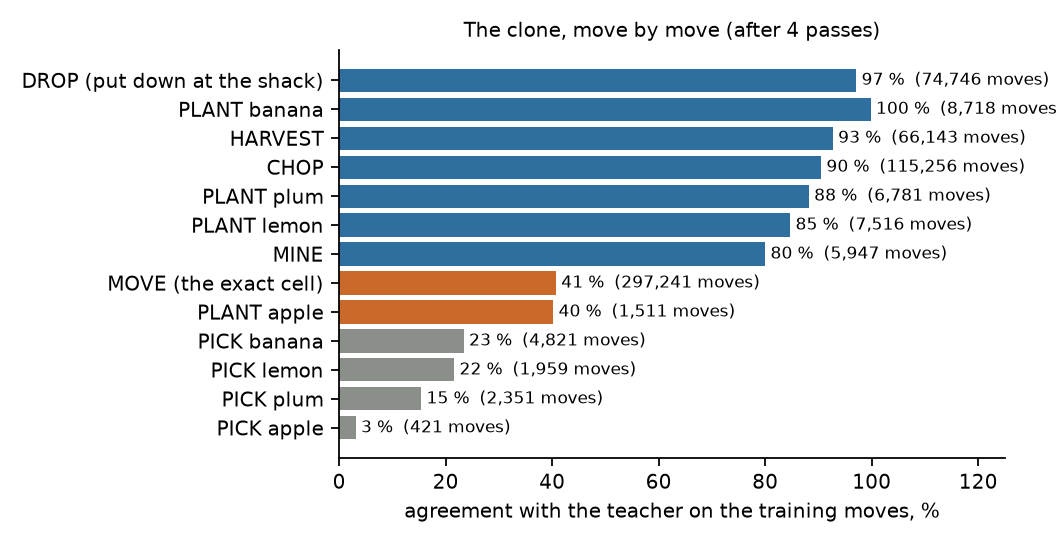
\includegraphics[width=\textwidth]{clone-verbs.png}
\caption{Agreement with the teacher, move by move. The routine moves are learned (drop, harvest, chop, plant); \emph{move to exactly this cell} is the hard one (one cell of up to 242); \emph{pick} (taking a fruit from the shack to plant it) is barely learned --- it is rare and depends on a plan the clone does not have.}
\label{fig:verbs}
\end{figure}

\begin{figure}[h]\centering
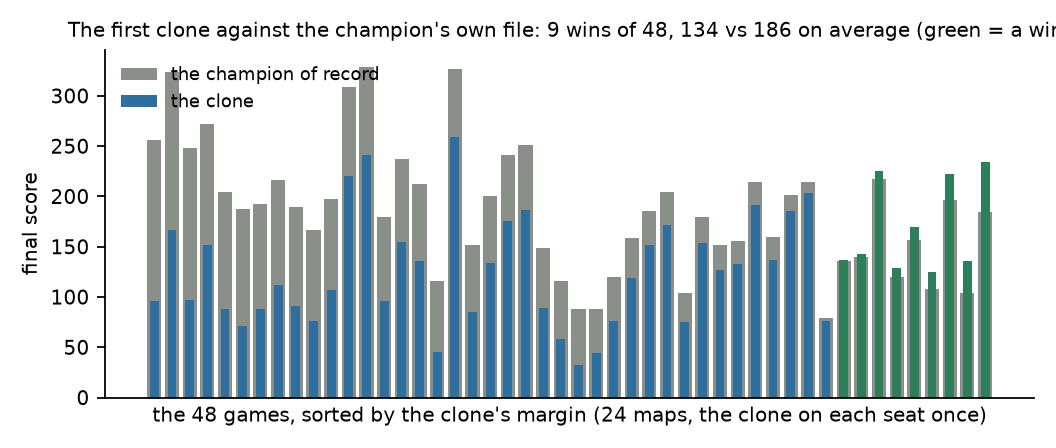
\includegraphics[width=\textwidth]{bench-clone.png}
\caption{The bench: the clone against the champion's own submitted file, 48 games. Grey bars are the champion's scores, the narrow bars the clone's; green marks the clone's wins. A random-move policy scores 13.5 on this bench.}
\label{fig:bench}
\end{figure}

\begin{figure}[h]\centering
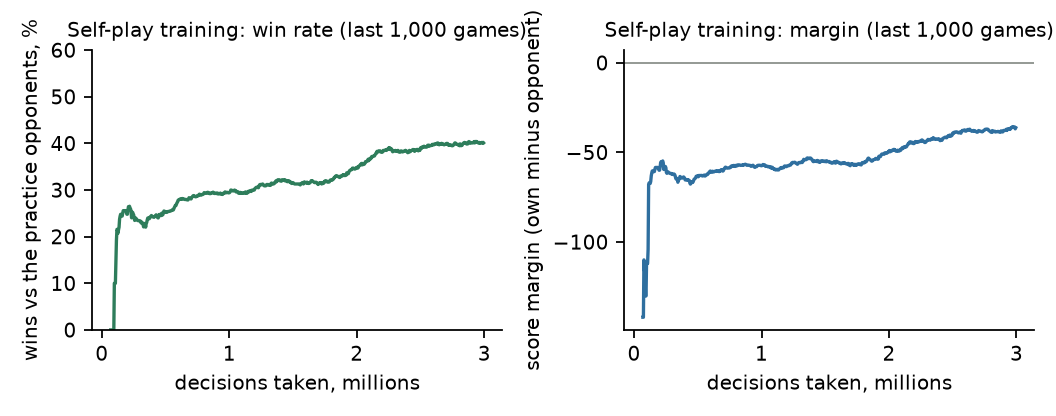
\includegraphics[width=\textwidth]{ppo-progress.png}
\caption{Self-play training so far (Phase 3), against the practice opponents (six hand-written bots and frozen copies of itself --- a harder mix than the champion alone). Both curves are over the last 1,000 finished games.}
\label{fig:ppo}
\end{figure}

\clearpage
\section{Where everything is}

Two places: the repository (code, cards, reports --- on \texttt{main}), and a data directory outside it (the big and the reproducible files).

\subsection*{The repository \fp{/home/tarstars/prj/troll_farm} (the same tree as my worktree \fp{.../troll_farm-local_claude_1})}
\begin{center}\small
\begin{tabular}{@{}L{7.2cm}L{8.2cm}@{}}
\toprule
path & what it is \\
\midrule
\fp{coordination/BOARD.md} & the one page to read: what is in motion, your queue \\
\fp{coordination/GOAL.md} & the target in full, and what I may and may not do without you \\
\fp{coordination/tasks/20260829-nn-bot-way-b.md} & the card: the design, every ruling, the log --- the record of this line \\
\fp{coordination/tasks/20260829-nn-bot-way-b-env.md}, \fp{...-dataset.md} & the two builders' contracts (Phases 1 and 2) \\
\fp{local_claude_1/nn-bot/ANALYSIS-2026-08-29.md} & the analysis you read before deciding \\
\fp{local_claude_1/nn-bot/OBS-PLANES.md}, \fp{ENV-API.md} & the signed interface: the 104 things the network sees; the environment's calls \\
\fp{rust/src/rl_full.rs} & the training environment (Rust): the game, 128 copies at once, the opponents \\
\fp{cgauto/rl_full_env.py} & its Python side: \texttt{rewards, info = env.step(actions)}; the replay checker \\
\fp{cgauto/train_level1_ppo.py} & the network itself (\texttt{SpatialActorCritic}) with its two heads \\
\fp{local_claude_1/nn-bot/nn_runtime.py} & one shared adapter: the board to planes, the masks, the command codec, the end rule \\
\fp{local_claude_1/nn-bot/build_dataset.py} & recorded games $\rightarrow$ the training set \\
\fp{local_claude_1/nn-bot/train_clone.py} & the training set $\rightarrow$ the clone \\
\fp{local_claude_1/nn-bot/train_ppo_full.py} & the clone $\rightarrow$ a better network by self-play \\
\fp{local_claude_1/nn-bot/bench.py} & the judge: a network against a compiled bot on real maps; prints any game turn by turn \\
\fp{local_claude_1/nn-bot/fake_full_env.py} & a stand-in environment for tests \\
\fp{local_claude_1/nn-bot/results/clone-2026-08-30-a/} & \textbf{the clone, its 48 games, the reports, a README for your read} \\
\fp{local_claude_1/reconstructions/fits/reconstruct.py} & the exact rebuild of a recorded game, turn by turn \\
\fp{tests/test_rl_full_env.py}, \fp{tests/test_train_ppo_full.py} & the tests (7 and 42) \\
\fp{docs/reports/2026-08-30-neural-network-line-progress.pdf} & this document \\
\bottomrule
\end{tabular}
\end{center}

\subsection*{The data directory \fp{/home/tarstars/nn-data/} (outside the repository)}
\begin{center}\small
\begin{tabular}{@{}L{6.2cm}L{9.2cm}@{}}
\toprule
path & what it is \\
\midrule
\fp{dataset-v400-2026-08-30/} & the training set: 817,811 decisions, 14\,MB, with checksums \\
\fp{clone-2026-08-30-a/} & the clone (\fp{clone-pilot.pt}), its training log, both bench reports and the 48 games (also copied into the repository) \\
\fp{ppo-2026-08-30-a/} & the self-play run: \fp{train.log} (one line per update), a snapshot every 250 updates \\
\fp{/home/tarstars/nn-venv/} & the Python used for all of this (3.11, PyTorch 2.13 for CPU) \\
\fp{/home/tarstars/prj/troll_farm/data/raw/games/} & the 24,973 recorded ladder games (7.1\,GB), the raw material \\
\bottomrule
\end{tabular}
\end{center}

\section{The structure of the data}\label{sec:data}

\textbf{A recorded game} (one file per game, 24,973 of them) holds the map at turn 0, both players' commands at every turn, and the referee's log. Positions and inventories are not stored per turn; \fp{reconstruct.py} replays both players' commands through our copy of the rules and checks every step against the referee's log --- on the 784 top-four games it disagrees with the referee on nothing.

\textbf{The training set} has three kinds of file in one directory:
\begin{itemize}[nosep,leftmargin=1.4em]
  \item \emph{states} (\fp{states-pilot.jsonl.gz}, 12.9\,MB): one compact line per turn --- every troll's position, talents and cargo, every tree's kind, size, health and fruit, both banks --- 58 bytes a turn, 224,400 turns;
  \item \emph{maps} (\fp{maps-pilot.json}): the 748 boards;
  \item \emph{labels} (\fp{labels-pilot.npz}, 1.3\,MB): what the teacher did. Two kinds of row. A \emph{plan row}, one per turn: which troll the player bought next (the number of that troll among 400 possibilities: speed 1--4, carry 1--5, harvest 0--3, chop 0--4; ``nothing'' when no purchase follows). A \emph{command row}, one per troll per turn: the move, as one number among $13 \times 242$ --- 13 kinds of action (move here, harvest, chop, drop, mine, plant four kinds, pick four kinds) over the 242 cells of the largest board; a \emph{move} is labelled with the cell the troll actually reached.
\end{itemize}
The network's input is not stored: it is built when needed, by the same Rust code the environment uses, as \textbf{104 planes of 11$\times$22 numbers} --- the cell types, the trees, the trolls and what they carry, distances to the shacks and to the nearest trees, the banks, the scores, the troll being decided, the troll being saved for. (Stored, this would be 20\,GB; built on the fly it costs 15\,ms a row.)

\textbf{Why 400 kinds of troll, not delineate's 144.} His network chose among speed 1--3, carry 1--4, harvest 0--2, chop 0--3. A count over the top four's 1,725 purchases found 267 outside that box --- Bubaptik buys speed-4 trolls in half of its purchases. The game caps nothing, so the vocabulary follows the teachers.

\begin{figure}[h]\centering
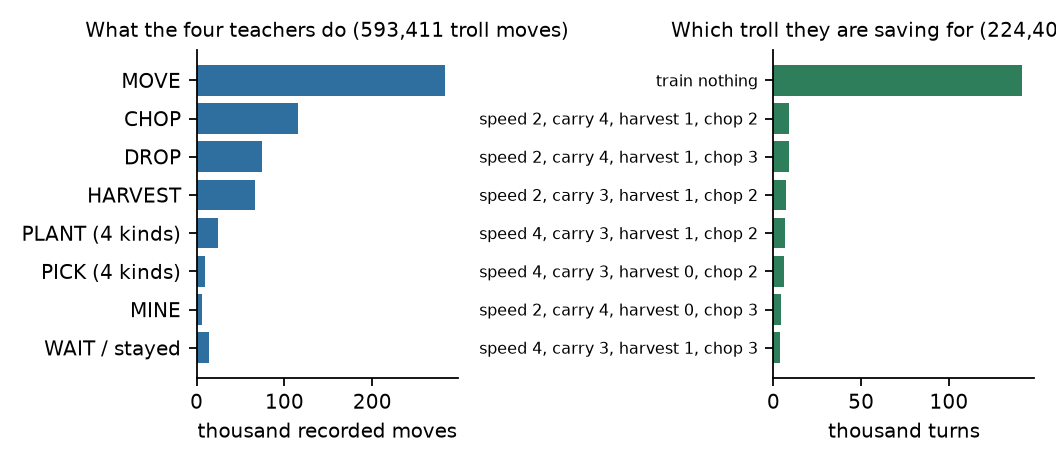
\includegraphics[width=\textwidth]{teachers.png}
\caption{What the training set contains. Left: the moves of the four teachers' trolls. Right: which troll they were saving for, turn by turn (``nothing'' after the last purchase of a game).}
\label{fig:teachers}
\end{figure}

\textbf{A checkpoint} (\fp{*.pt}) is four things: the network's weights, the optimizer's state, the settings it was trained with (including the vocabulary version \texttt{v400-2026-08-29} --- a checkpoint from another vocabulary is refused), and the step count.

\section{The structure of the programs}

\begin{verbatim}
 recorded games ---> reconstruct.py ---> build_dataset.py ---> training set
 (24,973 files)      (exact turn-by-turn)  (labels + states)    (14 MB)
                                                                    |
                          rl_full.rs (the game, x128)               v
                          + rl_full_env.py  <----------------- train_clone.py
                                |                                  |
                                v                                  v
                         train_ppo_full.py  <--- anchor ---   clone-pilot.pt
                          (self-play, PPO)
                                |
                                v
                      snapshots (*.pt) ---> bench.py ---> games, wins, scores
                                             (vs the champion's file)
                                |
                                v   (Phase 4, not built yet)
                      export -> int8 weights -> one Rust file -> the ladder
\end{verbatim}

\begin{center}\small
\begin{tabular}{@{}L{3.3cm}L{5.8cm}L{6.3cm}@{}}
\toprule
program & takes & gives \\
\midrule
\fp{reconstruct.py} & one recorded game & its exact state at every turn \\
\fp{build_dataset.py} & a directory of recorded games & the training set (states, maps, labels); a report; a self-check of every label \\
\fp{train_clone.py} & the training set, the Rust library & the clone checkpoint; a log per pass \\
\fp{rl_full.rs} + \fp{rl_full_env.py} & maps, opponents, actions & 128 games stepping together; rewards; the planes and masks; a replay checker \\
\fp{train_ppo_full.py} & a starting checkpoint, an anchor checkpoint, the environment & snapshots; one JSON line per update (win rate, margin, speed, how close to the anchor) \\
\fp{bench.py} & a checkpoint, a compiled bot, a map slice & 48 games with scores, purchases, ends; the games saved turn by turn \\
\fp{nn_runtime.py} & (shared by the three above) & the planes, the masks, the command codec, the exact ``can I train'' check, the end-of-game rule \\
\bottomrule
\end{tabular}
\end{center}

\textbf{The one decision every turn.} A turn is several decisions in a row: first \emph{which troll to save for} (one of 400, or nothing); then, for each own troll in order, \emph{what it does} (one of $13 \times 242$, most of them masked as impossible); then the turn executes for both players. The reward is the final score difference, paid once per turn on the last decision.

\section{The numbers so far}

\begin{center}\small
\begin{tabular}{@{}L{7.4cm}L{8.0cm}@{}}
\toprule
& \\
\midrule
The environment's check & 1,000 self-play games replayed through an independent rules copy: 0 disagreements, 0 illegal commands; 214 game-turns/s on the VM's 4 cores \\
The training set & 817,811 decisions (224,400 plan + 593,411 command) from 748 games; 0 labels outside the vocabulary; built in 1\,min\,42\,s \\
The clone, 4 passes & agreement with the teachers 74\,\% (which troll) and 65\,\% (what it does); Figure~\ref{fig:verbs} per move \\
The clone on the bench & 9 wins of 48 vs the champion's file (4 on seat 0, 5 on seat 1); 134 vs 186 points; 0 illegal commands, 0 timeouts; buys a troll at turn 1 in 44 games --- the teachers' harvest-carrying trolls, not the champion's chopper \\
Self-play, first hour & 615 updates, 2.5 million decisions; wins vs the practice mix 0 $\rightarrow$ 39\,\%; margin $-116 \rightarrow -41$; $\sim$670 decisions/s \\
This computer & 20 cores, no GPU: the network answers 17,000 boards/s in batches; the bottleneck is building the planes and running the opponents \\
\bottomrule
\end{tabular}
\end{center}

\section{How to read the clone's games}\label{sec:read}

\begin{verbatim}
cd /home/tarstars/prj/troll_farm
PYTHONPATH=. /home/tarstars/nn-venv/bin/python local_claude_1/nn-bot/bench.py \
    --read local_claude_1/nn-bot/results/clone-2026-08-30-a/\
bench-argmax-replays.jsonl --game 10
\end{verbatim}
\texttt{--game} is 1 to 48 (0 prints all). Each line is one turn: the champion's commands on the left, the clone's on the right. The table of games (map, seat, scores, purchases, how it ended) is \fp{bench-argmax.json}. Game 10 is a win (225 to 217); game 1 a loss with no purchase (76 to 167); game 34 has the clone's one long loop.

What I saw reading them: the second troll works like a teacher's --- walks to trees, harvests, plants lemons, brings fruit home; the first troll often \emph{picks a fruit from the shack and drops it back}, for stretches of ten or twenty turns --- copying without a purpose (pick and drop are 13\,\% of the recorded moves). It does not chop as a plan. Those two habits are what self-play must unlearn first.

\section{Risks and what would stop the line}

\begin{itemize}[nosep,leftmargin=1.4em]
  \item \emph{Self-play finds a hole in our copy of the game rather than a strategy.} Guard: samples of its games are replayed through the independent rules copy at every check.
  \item \emph{The practice opponents are not the ladder.} The bench uses the champion's real file; the target adds orchard~6; the ladder hour is the truth.
  \item \emph{Speed on the platform.} Our export kernel of July ran a 35,000-weight network in 7\,ms a turn; the limit is 50\,ms; the network stays small until measured.
  \item \emph{Dead conditions on the card:} no gain over the clone after 200 million decisions; or a hole in the engine --- then the run stops and the card says so.
\end{itemize}

\section*{The agents and the routine}
\emph{codex\_1} and \emph{claude\_1} build and reproduce each other's work on the VM; \emph{chatgpt\_1} audits on your instruction; I design, rule, integrate onto \texttt{main}, train on this computer and write to you. Every ruling and every number is in the card's log; the board's queue item~0 is the milestone note. No platform action has been taken since your word on 08-29 and none will be before Phase 4 and your prediction.

\end{document}
